\documentclass[12pt, a4paper, UTF8, fontset=windows]{ctexbook}
\usepackage{amsmath, amsthm, amssymb, amsfonts, bm, color, colortbl, fancyhdr, float, framed, geometry, graphicx, hyperref, lastpage, listings, mathrsfs, xcolor}


\linespread{1.5}
\definecolor{shadecolor}{RGB}{241, 241, 255}
\newcounter{problemname}
\newenvironment{problem}{\begin{shaded}\stepcounter{problemname}\par\noindent\textbf{Q\arabic{problemname}.}}{\end{shaded}\par}
\newenvironment{solution}{\par\noindent\textbf{Ans.}}{\par}

\geometry{left=20mm,right=20mm, top=20mm, bottom=22mm} % 页边距
\setlength{\headheight}{15pt}
\pagestyle{fancy} % 设置页脚页眉
\rhead{Assignment2} % 页眉右边
% \noindent % 取消首段缩进

\definecolor{mygreen}{rgb}{0,0.6,0}
\definecolor{mygray}{rgb}{0.5,0.5,0.5}
\definecolor{mymauve}{rgb}{0.58,0,0.82}
% 代码设置
\lstset{ 
    backgroundcolor=\color{white},      % choose the background color
    basicstyle=\footnotesize\ttfamily,  % size of fonts used for the code
    columns=fullflexible,
    tabsize=4,
    breaklines=true,               % automatic line breaking only at whitespace
    captionpos=b,                  % sets the caption-position to bottom
    commentstyle=\color{mygreen},  % comment style
    keywordstyle=\color{blue},     % keyword style
    stringstyle=\color{mymauve}\ttfamily,  % string literal style
    frame=single,
    rulesepcolor=\color{red!20!green!20!blue!20},
    language=c++,
    xleftmargin=3em,
    xrightmargin=3em
}


\begin{document}

\cfoot{\thepage\ / \pageref{LastPage}} % 页眉中间位添加内容:页码/总页码

\thispagestyle{empty}

\begin{figure}[t]
    \centering
    
\includegraphics[width=6cm]{../../src/images/logo.jpg}
\end{figure}

\vspace*{\fill}
    \begin{center}
        \Huge\textbf{Assignment2}
    \end{center}
\vspace*{\fill}

\begin{table}[b]
    \centering
    \large
    \begin{tabular}{ll}
        \textbf{Course:} & Computer Network \\
        \textbf{Name:} & Xiang Lei (雷翔) \\
        \textbf{Student ID:} & 2053932 \\
        \textbf{Date:} & November 2023 \\
    \end{tabular}
\end{table}

\newpage

\setcounter{page}{1} % 页码从当前页开始

\begin{problem}
    ARQ

    Consider the data transmission from sender A to receiver B via the Go-Back-N (with NAK)
    protocol with a large window size N (so that packet transmissions will not be limited by the
    window size).

    a) Fill in the boxes of the figure below. Write the packet number in the form of Px, and the
    response in the form of ACKx or NAKx. (14 points)
    
    b) Write the corresponding actions (A for Accept, DD for discard as duplicates, DE for
    discard as error) for each packet at the receiver end. (6 points)
\end{problem}

\begin{solution}

    % image
    \begin{figure}[H]
        \centering
        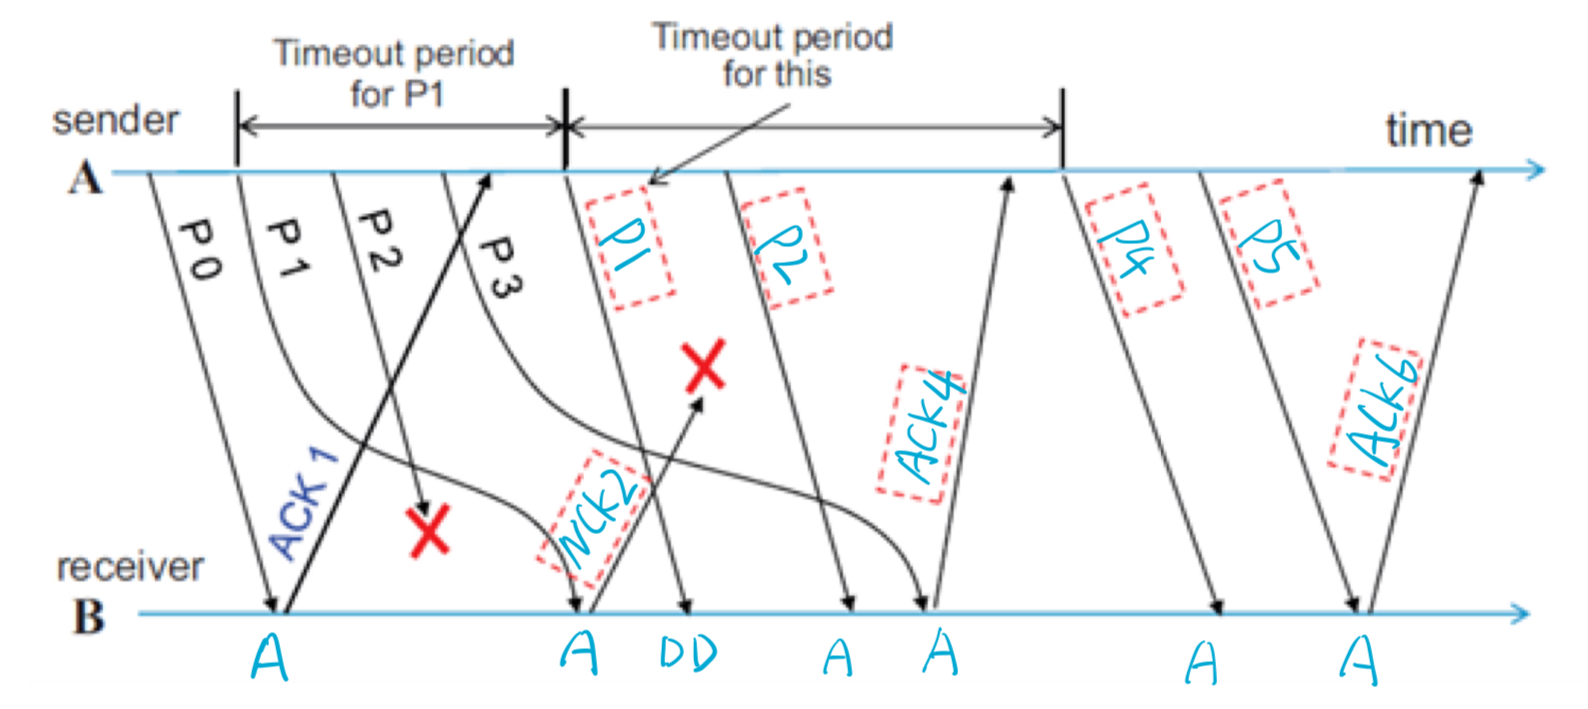
\includegraphics[width=0.99\textwidth]{../src/Q1.png}
    \end{figure}

\end{solution}


\begin{problem}
    Medium Access Control (25 points, 5 points each)
    
    Briefly answer the following questions in your own words.

    a) Describe the CSMA/CA mechanism used in IEEE 802.11 (WiFi). You may draw a dia-
    gram, describe in words, or write pseudo code for this.
    
    b) Why can’t we use CSMA/CD in wireless LAN?
    
    c) Why do we need the RTS-CTS mechanism?
    
    d) How does a bridge learn the hosts in a LAN? (Hint: Read Chapter 4.8.2 and 4.8.3 in the
    textbook)
    
    e) What are the differences between a bridge/switch and a hub? (Hint: Read Chapter 4.8.4
    in the textbook)
\end{problem}

\begin{solution}
    a)
    % 当源站要发送数据帧时,它监听信道,如果信道空闲,它就发送数据;
    % 否则它等待,直至信道空闲。当信道从忙态变为空闲态时,任何一个站要发送数据帧,
    % 不仅要等待一个时间间隔,还要进入争用窗口,计算随机退避时间以便再次接入信道。
    When a source station intends to transmit a data frame, it listens to the channel. If the channel is idle, 
    it sends the data; otherwise, it waits until the channel becomes idle. When the channel transitions from busy to idle, 
    any station intending to transmit a data frame not only needs to wait for a time interval but also enters a contention window. 
    It calculates a random backoff time to attempt accessing the channel again.
    
    \begin{figure}[H]
        \centering
        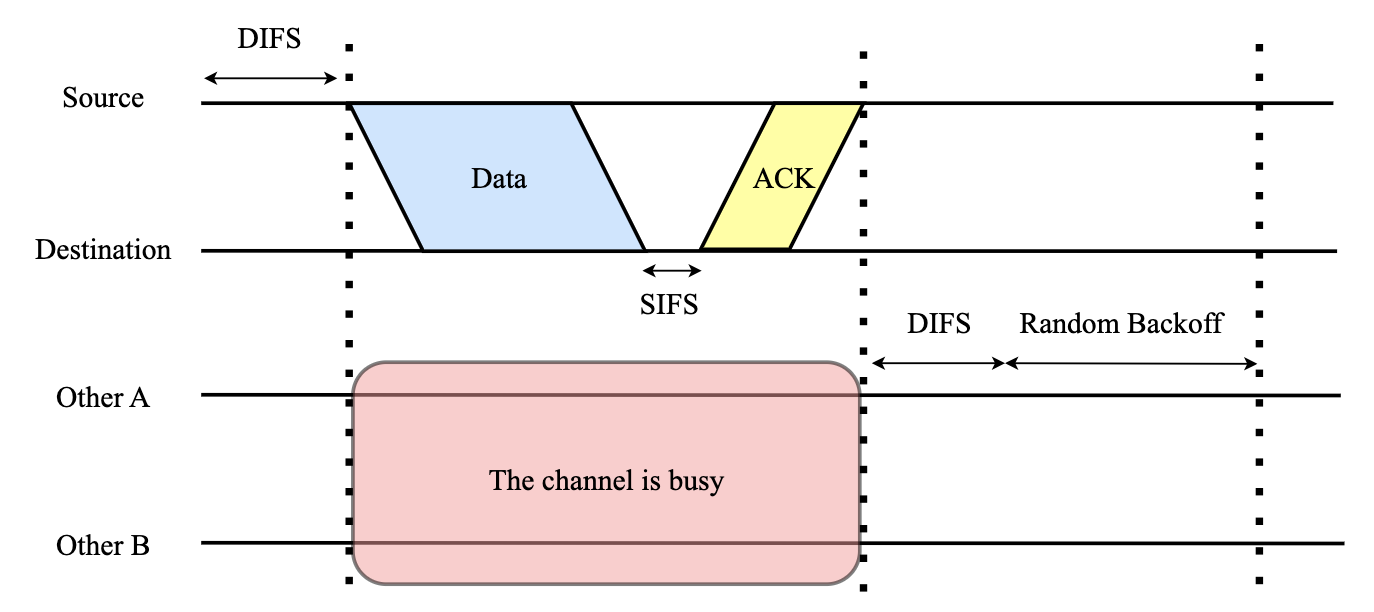
\includegraphics[width=0.99\textwidth]{../src/Q2-a.png}
    \end{figure}

    b)
    % 第一点:无限网卡上接受信号的强度往往会远小于发送信号的强度,如果要在无线网卡上实现碰撞检测,对硬件要求很高;
    % 第二点:无线电窗玻存在隐蔽站问题,进行碰撞检测的意义不大。
    Firstly, the received signal strength on wireless network cards is often much weaker than the transmitted signal strength. Achieving collision detection on wireless network cards requires high hardware demands. 
    
    Secondly, there is the hidden station problem in radio windows, making collision detection less meaningful.

    c)
    % RTS/CTS 请求发送/清除发送,主要用于解决隐藏站问题。
    % RTS/CTS 机制的基本思想是:发送方在发送数据前,先发送一个短的RTS帧给接收方,
    % 接收方收到后,如果空闲,则回复一个CTS帧给发送方,发送方收到CTS帧后,才发送数据帧。
    RTS/CTS (Request to Send/Clear to Send) is primarily employed to address the hidden station problem. The fundamental idea behind the RTS/CTS mechanism is that, before transmitting data, the sending station first sends a short RTS frame to the receiving station. Upon receiving the RTS frame, if the channel is idle, the receiving station replies with a CTS (Clear to Send) frame to the sending station. Only after the sending station receives the CTS frame does it proceed to send the data frame.

    \begin{figure}[H]
        \centering
        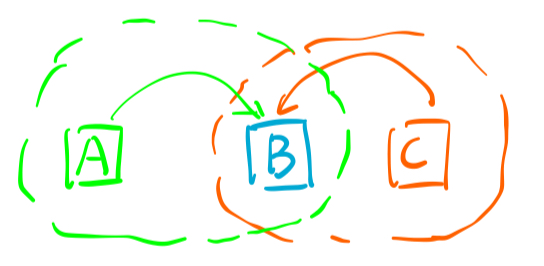
\includegraphics[width=0.6\textwidth]{../src/Q2-c.png}
    \end{figure}

    d)
    % 网桥如何了解局域网中的主机?
    The bridge creates a hash table entry for each machine, indicating the corresponding output port. Initially, when bridges are powered up and the hash tables are empty, they use a flooding algorithm. Incoming frames for unknown destinations are broadcast to all ports (except the incoming port). As bridges learn the locations of destinations over time, flooding is reduced, and frames are forwarded only to the proper port. To handle dynamic topologies, hash table entries include the arrival time of frames, enabling updates based on the last time a frame from a specific machine was seen. This ensures effective address learning and adaptation to changing network configurations.

    e)
    % 网桥/交换机和集线器之间有什么区别?
    \textbf{Operational Layer}

        Bridge/Switch: Operates at the Data Link Layer (Layer 2) of the OSI model. Examines and makes decisions based on the MAC addresses in the frame headers.
    
        Hub: Operates at the Physical Layer (Layer 1) of the OSI model. Functions as a simple repeater, broadcasting incoming frames to all connected devices.

    \textbf{Collision Domain}

        Bridge/Switch: Each port on a bridge/switch is typically its own collision domain, isolating traffic and reducing collisions. Full-duplex connections further eliminate collisions.
        
        Hub: All devices connected to a hub share the same collision domain. If two devices transmit data simultaneously, a collision occurs, and CSMA/CD (Carrier Sense Multiple Access with Collision Detection) is used to handle collisions.

    \textbf{Performance}

        Bridge/Switch: Offers better performance compared to hubs. Bridges and switches can make intelligent forwarding decisions, reducing unnecessary traffic and collisions.
        
        Hub: Can lead to network congestion and collisions, especially in larger networks, as all devices connected to the hub share the same bandwidth.

    \textbf{Use Cases}

        Bridge/Switch: Suitable for modern networks where performance and efficient use of bandwidth are essential. Commonly used in Ethernet networks.
    
        Hub: Less common in modern networks due to performance limitations. Typically used in simpler, smaller-scale setups.
\end{solution}

\newpage

\begin{problem}
    IP Addressing (10 points)

    Briefly answer the following questions.
    
    a) For a network with IP address 192.168.8.0/26, how many host IP addresses can be assigned
    in this network? (3 points)
    
    b) With respect to the number of destinations, IP addresses can be categorized into three
    types. What are they? Give an example for each type of addresses. (4 points)
    
    c) ARP is an aiding protocol for IP. Describe in your own words how ARP request and ARP
    reply works. (3 points)    
\end{problem}

\begin{solution}
    
    a) For IP address 192.168.8.0/26, there are 62 host IP addresses can be assigned in this network.
    The first 26 bits are network bits, and the last 6 bits are host bits.
    So the number of host IP addresses is $2^6 - 2 = 62$. (2 IP addresses are reserved for broadcast and network)

    b) IP addresses can be categorized into three types: Unicast Address, Multicast Address, and Broadcast Address.

    Unicast Address: Used to send a message to a single host. $e.g.$ 192.168.1.1

    Multicast Address: Used to send a message to a group of hosts. $e.g.$ 224.0.0.1

    Broadcast Address: Used to send a message to all hosts on a network. $e.g.$ 192.168.1.255

    c) ARP contains the mapping between each host's IP address and MAC address. 
    
    The ARP request and ARP reply works as follow:

    ARP request: When a host wants to send a message to another host, it will first check the ARP cache to see if the MAC address of the destination host is in the cache.
    If the MAC address is in the cache, the host will send the message to the destination host directly.
    If the MAC address is not in the cache, the host will broadcast an ARP request message to all hosts on the network.

    ARP reply: When a host receives an ARP request message, it will check if the IP address in the message is its own IP address.
    If the IP address is its own IP address, the host will send an ARP reply message to the sender of the ARP request message.
    Then the sender will add the IP address and MAC address in the ARP reply message to its ARP cache.
\end{solution}

\newpage

\begin{problem}
    Routing: Dijkstra (20 points)

    Consider the network topology as follow.

    a) Describe the Dijkstra algorithm with pseudo code. (5 points)

    b) Find the shortest path from node A to all the other nodes in the network with the Dijkstra
    algorithm. Make sure you show all your steps (with the table!). (10 points)

    c) Consider a networking condition in which you are asked to write an algorithm to find the
    most reliable path, i.e., the path with the least Bit Error Rate (BER). Assume each link
    in the network has a BER (in the range of 0 and 1) that is independent of other links.
    Can we directly use Dijkstra algorithm? If not, how to change it to solve this problem?
    (5 points)
\end{problem}

\begin{solution}
    a)

    \begin{lstlisting}[language=python]
    function Dijkstra(G, s):
        """
        G: graph
        s: source node
        """
        for each vertex v in G:  # Initialization
            dist[v] = infinity
            prev[v] = undefined

        dist[s] = 0
        Q = G.V

        while Q is not empty:
            # find dist[u] where u belongs to Q
            u = min(Q, key=lambda v: dist[v])
            Q.remove(u)

            for each neighbor v in u:
                item = dist[u] + length(u, v)
                if item < dist[v]:
                    dist[v] = item
                    prev[v] = u

        return dist, prev
    \end{lstlisting}

    b)

    \begin{table}[H]
        \centering
        \begin{tabular}{c|c|c|c|c|c|c}
            \hline
            \rowcolor{gray!30}
            Step & set N & D(B), p(B) & D(C), p(C) & D(D), p(D) & D(E), p(E) & D(F), p(F) \\
            \hline
            0 & A & 4, A & 1, A & $\infty$ & $\infty$ & $\infty$ \\
            \hline
            1 & A, C & 3, C & 1, A & $\infty$ & 4, C & $\infty$ \\
            \hline
            2 & A, C, B & 3, C & 1, A & 8, D & 4, C & 12, B \\
            \hline
            3 & A, C, B, E & 3, C & 1, A & 5, E & 4, C & 7, E \\
            \hline
            4 & A, C, B, E, D & 3, C & 1, A & 5, E & 4, C & 6, D \\
            \hline
            5 & A, C, B, E, D, F & 3, C & 1, A & 5, E & 4, C & 6, D \\
            \hline
        \end{tabular}
    \end{table}

    D(B) = 3, A -> C -> B

    D(C) = 1, A -> C

    D(D) = 5, A -> C -> E -> D

    D(E) = 4, A -> C -> E

    D(F) = 6, A -> C -> E -> D -> F

    c) No, we can't directly use Dijkstra algorithm.

    Dijkstra algorithm is used to find the shortest path in a graph where the weight of each edge is non-negative. 
    The shortest path means the sum of the weights of the edges on the path is minimum. However, in this problem,
    we want to find the most reliable path, i.e., the path with the least Bit Error Rate (BER). 
    The most reliable path means the product of the weights of the edges on the path is minimum.
    So we must change the algorithm to find the most reliable path.

    \begin{lstlisting}[language=python]
    function Dijkstra(G, s):
        """
        G: graph
        s: source node
        """
        for each vertex v in G:  # Initialization
            M_UBER = 1  # bigger M_UBER -> better result
            prev[v] = undefined

        M_UBER[s] = 1
        Q = G.V

        while Q is not empty:
            # find M_UBER[u] where u belongs to Q
            u = max(Q, key=lambda v: M_UBER[v])
            Q.remove(u)

            for each neighbor v in u:
                item = M_UBER[u] * (1 - BER(u, v))
                if item > M_UBER[v]:
                    M_UBER[v] = item
                    prev[v] = u

        return dist, prev
    \end{lstlisting}
\end{solution}


\begin{problem}
    Routing: Bellman-Ford (10 points)

    Consider the same network topology as in Question 4, and find the shortest path to node A
    with the Bellman-Ford algorithm. Update Order B → C → D → E → F. Make sure you
    show all your steps (with the table!).
\end{problem}

\begin{solution}
    \begin{table}[H]
        \centering
        \begin{tabular}{c|c|c|c|c|c}
            \hline
            \rowcolor{gray!30}
            Cycle & n(B), D(B) & n(C), D(C) & n(D), D(D) & n(E), D(E) & n(F), D(F) \\
            0 & $\cdot$, $\infty$ & $\cdot$, $\infty$ & $\cdot$, $\infty$ & $\cdot$, $\infty$ & $\cdot$, $\infty$ \\
            \hline
            1 & A, 4 & A, 1 & B, 9 & C, 4 & E, 7 \\
            \hline
            2 & C, 3 & A, 1 & E, 5 & C, 4 & D, 6 \\
            \hline
            3 & C, 3 & A, 1 & E, 5 & C, 4 & D, 6 \\
            \hline
        \end{tabular}
    \end{table}

    D(B) = 3, B -> C -> A

    D(C) = 1, C -> A

    D(D) = 5, D -> E -> C -> A

    D(E) = 4, E -> C -> A

    D(F) = 6, F -> D -> E -> C -> A
\end{solution}


\begin{problem}
    QoS (15 points)
    
    Give real-world examples for the following scheduling schemes.
    
    a) FIFO Queue (4 points)

    b) Priority Queue (4 points)

    c) Round Robin (4 points)

    d) Weighted Fair Queue (WFQ) (3 points)
\end{problem}

\begin{solution}

    % 大学食堂排队,第一个排队的人先打饭,第二个排队的人再打饭,以此类推。
    a) Consider an university cafeteria. the first person who queued up will get the food first, the second person who queued up will get the food second, and so on.
    
    % 医院急诊室,病情严重的优先看病。
    b) Consider an hospital. The patient with serious illness will be treated first. 
    
    % 部分企业面试,在无领导小组面试环节,每个人都有平等的机会去发言。
    c) Consider a job interview. In the group interview, each person has an equal opportunity to speak.
    % 在计算机网络,Round Robin 是一种公平的调度算法;
    % 当多个数据包同时到达路由器,并需要通过同一个输出端口转发时,Round Robin 调度算法保证每个数据包都有机会被转发,且每个数据包被转发的时间间隔相对均衡
    In computer networks, Round Robin is a fair scheduling algorithm. When multiple packets arrive at the router at the same time and need to be forwarded through the same output port, 
    the Round Robin scheduling algorithm ensures that each packet has a chance to be forwarded, and each packet is forwarded at a relatively balanced interval
    
    % WFQ 以 bit 为单位进行调度,按队列权重来分配每个流应占有出口的带宽
    % 防止某些流占用过多的带宽,导致其他流的带宽不足
    d) In Weighted Fair Queue (WFQ), the scheduling is based on bits. The bandwidth of each flow is allocated according to the queue weight.
    It prevents some flows from occupying too much bandwidth, which leads to insufficient bandwidth of other flows.
\end{solution}


\end{document}